
\documentclass{standalone}
    \usepackage{tikz}
    \usetikzlibrary{arrows,decorations.pathmorphing,backgrounds,positioning,fit} 
    \usetikzlibrary{shapes.geometric}
    \def\radius{1mm}
    \usetikzlibrary{intersections}
    \usepackage{tkz-euclide}
    \usetkzobj{all}

    
    \usepackage{subcaption}    
    \begin{document}
    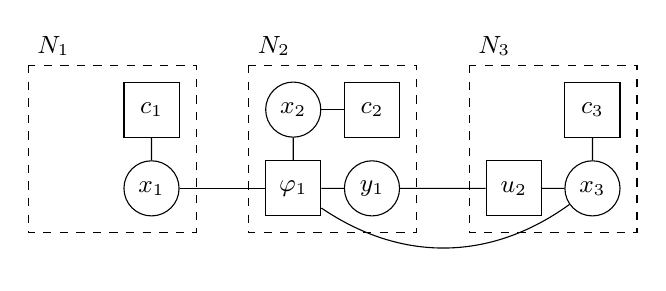
\begin{tikzpicture}[scale=0.8]%node distance=1cm]
        \small
        \tikzstyle{var} = [circle,draw,minimum height=0.7cm]
        \tikzstyle{fac} = [rectangle,draw,minimum width=0.7cm,minimum height=0.7cm]
        \tikzstyle{sen} = [diamond,draw,minimum width=0.7cm,minimum height=0.7cm]
        
        % actuator #1
        \node[fac,draw=none] (zero) at (0,0) {};
        \node[fac,right of=zero] (c1) {$c_1$};
        \node[var,below of=c1] (x1) {$x_1$};
        \coordinate[above left of=zero,node distance=0.8cm] (n11);
        \coordinate[below right of=x1,node distance=0.8cm] (n12);
        \draw[dashed] (n11) rectangle (n12) node[pos=0,anchor=south west] {$N_1$};		
        \path (c1) edge (x1);
  
        % actuator #2
        \node[var, right of=c1, node distance = 1.8cm] (x2) {$x_2$};
        \node[fac,right of=x2] (c2) {$c_2$};
        \node[fac,below of=x2] (f1) {$\varphi_1$};
        \node[var,right of=f1] (y1) {$y_1$};
        \path (x2) edge (c2);
        \path (x2) edge (f1);
        \path (f1) edge (y1);
        \coordinate[above left of=x2,node distance=0.8cm] (n21);
        \coordinate[below right of=y1,node distance=0.8cm] (n22);
        \draw[dashed] (n21) rectangle (n22) node[pos=0,anchor=south west] {$N_2$};
  
        % actuator #3
        \node[fac, right of=y1, node distance=1.8cm] (u2) {$u_2$};
        \node[var, right of=u2] (x3) {$x_3$};
        \node[fac, above of=x3] (c3) {$c_3$};
        \node[fac, above of=u2,draw=none] (phantom) {};
        \path (c3) edge (x3);
        \path (u2) edge (x3);
        \coordinate[above left of=phantom,node distance=0.8cm] (n31);
        \coordinate[below right of=x3,node distance=0.8cm] (n32);
        \draw[dashed] (n31) rectangle (n32) node[pos=0,anchor=south west] {$N_3$};
              
        % communication links between nodes
        \path[bend right=35] (f1) edge (x3);
        \path[bend left=0] (y1) edge (u2);
        \path[bend left=0] (x1) edge (f1);
      \end{tikzpicture}

\end{document}
